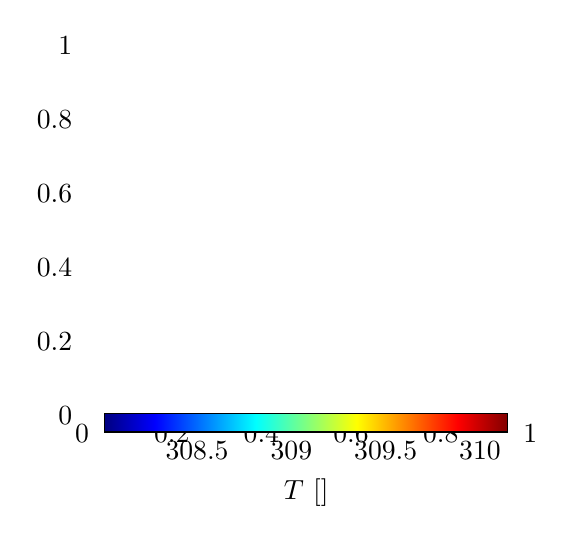
\begin{tikzpicture}
    \begin{axis}[
        colorbar,
        colormap/jet, % Choose the colormap you prefer
        % axis equal image,
        enlargelimits=false,
        point meta max=310.14813232421875,
        point meta min=308.0091857910156,
        colorbar horizontal,
        axis line style = {draw=none},
        tick style = {draw=none},
        xtick = \empty, ytick = \empty,
        colorbar style={
            xlabel = {$T$ [\si{\kelvin}]},
            height=0.05*\pgfkeysvalueof{/pgfplots/parent axis height},
            width=0.9*\pgfkeysvalueof{/pgfplots/parent axis width},
            at={(0.5,-0.02)}, % Adjust the position to center vertically
            anchor=center, % Adjust the anchor point
        },
        width=0.6\textwidth
    ]
        \addplotgraphicsnatural[xmin=0, xmax=1, ymin=0, ymax=1]{graphics/feelpp/feelpp-benchmark-heatfluid-resheat.png}

        \draw[->] (0.8, 0.9) -- (0.8, 0.8) node[midway, anchor=west] {$\vct{g}$};

        \draw[->, red] (0.1, 0.1) -- (0.2, 0.1) node[pos=1, anchor=north] {$x$};
        \draw[->, green!60!black] (0.1, 0.1) -- (0.1, 0.2) node[pos=1, anchor=east] {$y$};
        \draw[blue] (0.1, 0.1) node {$\odot$};
        \draw[blue] (0.1, 0.1) node[anchor=north east] {$z$};
    \end{axis}
\end{tikzpicture}